% Perfil em S da move_joints: posição e velocidade normalizadas (precisa de \usepackage{pgfplots})
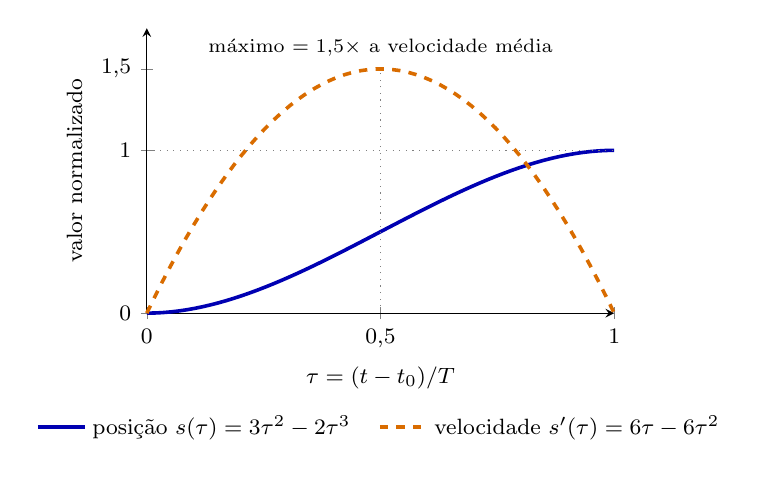
\begin{tikzpicture}
  \begin{axis}[width=0.62\textwidth, height=5.2cm,
      xmin=0, xmax=1, ymin=0, ymax=1.75,
      xlabel={$\tau = (t - t_0)/T$}, ylabel={valor normalizado},
      xtick={0, 0.5, 1}, ytick={0, 1, 1.5},
      yticklabels={$0$, $1$, $1{,}5$}, xticklabels={$0$, $0{,}5$, $1$},
      legend style={at={(0.5,-0.32)}, anchor=north, font=\footnotesize, draw=none, fill=none, legend columns=2, /tikz/every even column/.append style={column sep=8pt}},
      tick label style={font=\footnotesize}, label style={font=\footnotesize},
      axis lines=left, clip=false]
    \addplot[blue!70!black, line width=1.3pt, domain=0:1, samples=60] {3*x^2 - 2*x^3};
    \addlegendentry{posição $s(\tau) = 3\tau^2 - 2\tau^3$}
    \addplot[orange!85!black, line width=1.3pt, dashed, domain=0:1, samples=60] {6*x - 6*x^2};
    \addlegendentry{velocidade $s'(\tau) = 6\tau - 6\tau^2$}
    \addplot[gray, thin, dotted] coordinates {(0,1) (1,1)};
    \addplot[gray, thin, dotted] coordinates {(0.5,0) (0.5,1.5)};
    \node[font=\scriptsize, anchor=south] at (axis cs:0.5,1.52) {máximo $= 1{,}5\times$ a velocidade média};
  \end{axis}
\end{tikzpicture}